% interactapasample.tex
% v1.05 - August 2017

\documentclass[]{interact}

\usepackage{epstopdf}% To incorporate .eps illustrations using PDFLaTeX, etc.
\usepackage[caption=false]{subfig}% Support for small, `sub' figures and tables
%\usepackage[nolists,tablesfirst]{endfloat}% To `separate' figures and tables from text if required
%\usepackage[doublespacing]{setspace}% To produce a `double spaced' document if required
%\setlength\parindent{24pt}% To increase paragraph indentation when line spacing is doubled

\usepackage[longnamesfirst,sort]{natbib}% Citation support using natbib.sty
\bibpunct[, ]{(}{)}{;}{a}{,}{,}% Citation support using natbib.sty
\renewcommand\bibfont{\fontsize{10}{12}\selectfont}% To set the list of references in 10 point font using natbib.sty
\usepackage{float}

%\usepackage[natbibapa,nodoi]{apacite}% Citation support using apacite.sty. Commands using natbib.sty MUST be deactivated first!
%\setlength\bibhang{12pt}% To set the indentation in the list of references using apacite.sty. Commands using natbib.sty MUST be deactivated first!
%\renewcommand\bibliographytypesize{\fontsize{10}{12}\selectfont}% To set the list of references in 10 point font using apacite.sty. Commands using natbib.sty MUST be deactivated first!

\theoremstyle{plain}% Theorem-like structures provided by amsthm.sty
\newtheorem{theorem}{Theorem}[section]
\newtheorem{lemma}[theorem]{Lemma}
\newtheorem{corollary}[theorem]{Corollary}
\newtheorem{proposition}[theorem]{Proposition}

\theoremstyle{definition}
\newtheorem{definition}[theorem]{Definition}
\newtheorem{example}[theorem]{Example}

\theoremstyle{remark}
\newtheorem{remark}{Remark}
\newtheorem{notation}{Notation}

\begin{document}

\title{Chess Predictor: Using AdaBoost to Predict Chess Games}

\author{
\name{Matthew Ardizzone, Adam Cogdell, Michael York}
}

\maketitle

\begin{center}
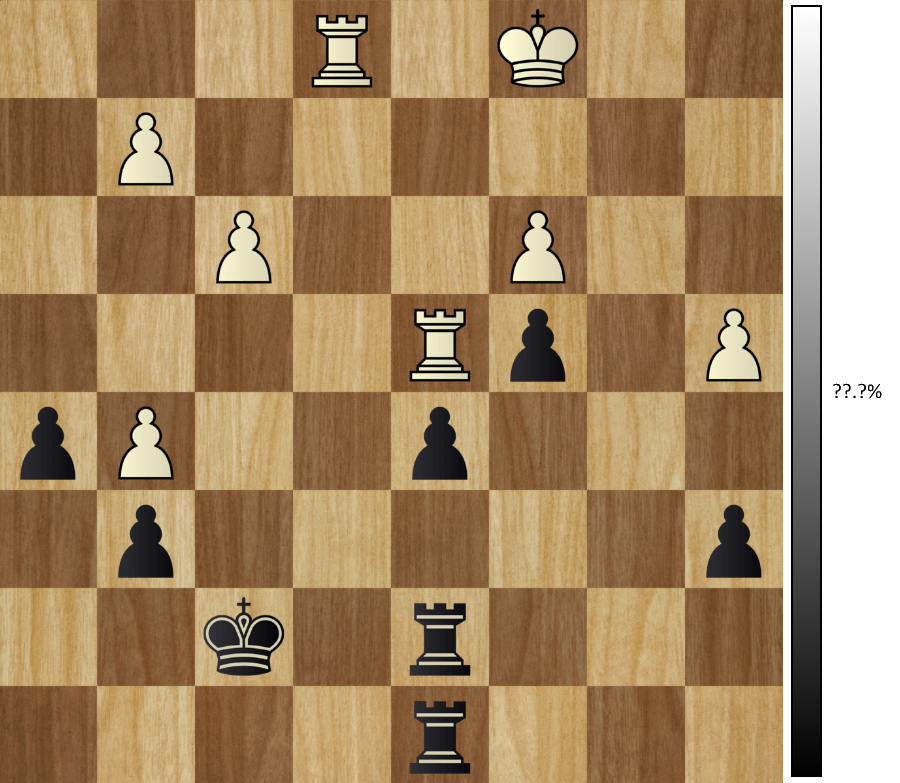
\includegraphics[scale=0.25]{intro.png}
\end{center}

\begin{abstract}
    Chess is a classic test bed in computing for evaluation of algorithms and engines. Using adaptive boosting techniques in machine learning, we are able to predict the outcome of chess games, a difficult task for classical machine learning algorithms due to the small-scale decisions and large-scale strategy that this game involves and inspires.
\end{abstract}

\section{Introduction}
Chess is perhaps one of the most well-known board games in the world. Since computing technologies have been able to, have people used them to predict the best moves in games.$^1$ For this project, we wanted to answer the question: can a model be created that predicts the outcome of a chess game simply based on a subset of moves that have occurred?

\subsection{Chess Engines}
A chess engine is a computer program that will play chess, either against a player or another engine. These engines have the ability to effectively pick the best move, through various methods. One of these engines, which is one of the most popular available, is known as Stockfish.$^2$ Engines have a particular ability to look ahead by iteratively looking at move possibilities for both players, something out of the scope of this project. To be clear, this project was \textit{not} created in order to be a chess engine. It is important to note that the only classes being considered for our model are ‘black wins’ and ‘white wins’, having removed any incomplete or tied games.

\subsection{Definitions}
To explain how our model works, we must first define a few terms. A \textit{turn} in chess is a pair of sequential moves made by both players. A \textit{move} is any change to the board state made by a player. For a given dataset, we have the ability to filter the dataset such that only games with \textit{n} turns or more remain. Increasing this \textit{turn threshold} reduces the number of samples available for learning, but gives the model more information per sample. Choosing this threshold proved to be a crucial step in tuning our model, since the quantity vs. quality trade-off it manifested was directly linked to performance.

\section{Dataset}

\begin{figure}[H]
\centering
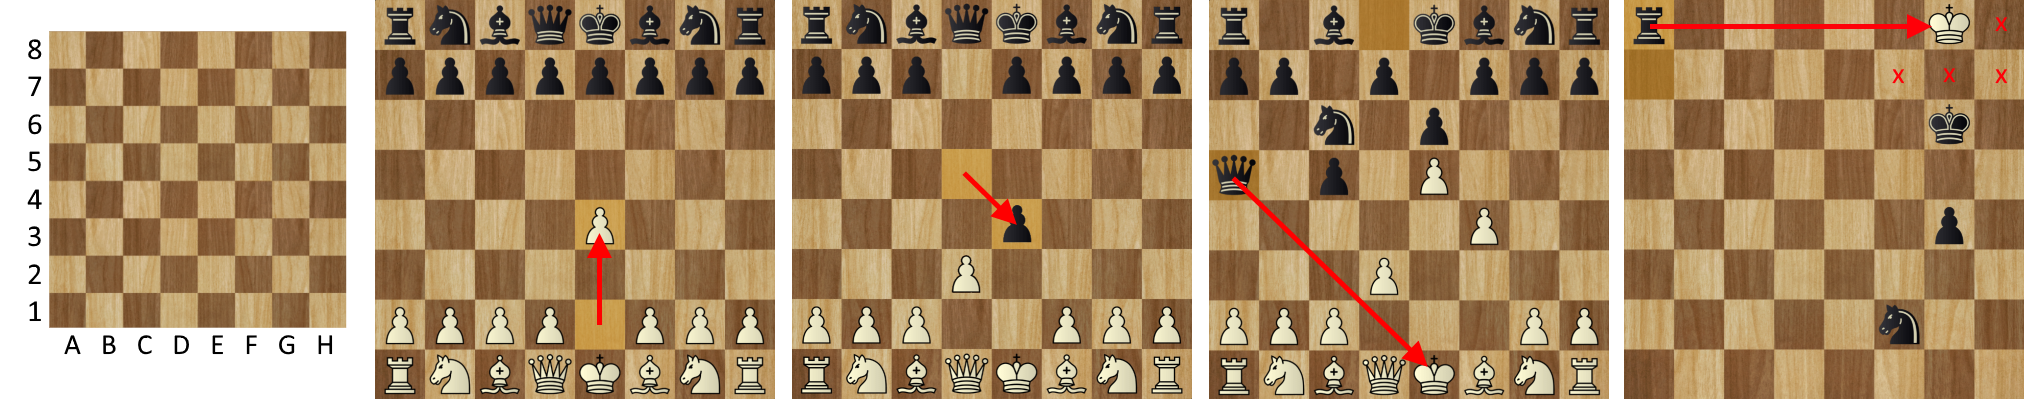
\includegraphics[scale=0.3]{chessmoves.png}
\caption{In this figure, we take a closer look at Portable Game Notation, or PGN. In the first image, the standard chess board coordinate system is drawn. Columns, or “files,” are notated with letters in alphabetical order from left to right. Rows, or “ranks,” are notated with numbers in counting order from bottom up. White’s pieces are placed in ranks 1-2 while black’s pieces are placed in ranks 7-8. In the second image, white moves its pawn on the E file to the 4th rank, and thus this move is notated e4. Any time a piece other than a pawn moves, a letter associated with that piece is placed first (For example if it were a king, it would be Ke4, a Queen Qe4 and so on). In the third image, black’s pawn on the D file is shown taking white’s pawn on the E file. Taking the opponent’s piece is notated with an ‘x.’ Thus this move is notated dxe4. In the fourth image, black’s queen moves to the a5 square, checking white’s king. When check occurs, a ‘+’ is added at the end of the move. This example is notated Qa5+. In the fifth image, white’s king has been checkmated by black’s rook, as it is both in check and has no other moves left. When checkmate occurs, a ‘\#' is added at the end of the move. This example is notated Rh1\#.}
\end{figure}

In order to create an effective learning model for this, we needed a dataset of chess games with their outcomes. A large database of chess games with their moves is available in the public domain thanks to lichess, an online open source chess gaming platform.$^3$ Without the generous public domain offering of chess games, this model would not have been possible to create, so we thank lichess for their offering.

The data made available by lichess was provided in PGN (Portable Game Notation) movetext format (see figure 1, above), stored in data as one large string, containing all the moves of the game in order and separated by spaces. We built a short parsing utility using the python-chess library which would convert a space-separated list of these chess moves to integers which were much easier to work with when building our model. We chose to encode each move as a concatenation of the ASCII codes of each character within that move. For example, The move ‘Na5’ is extracted from the large string and made its own distinct element. Then, the string is converted to the character array [ ‘N’, ‘a’, ‘5’ ]. Then, each character is converted to ASCII format   ([ ‘N’, ‘a’, ‘5’ ] becomes [ 78, 97, 53 ]). Finally, the character array’s elements are concatenated to form a single numerical value, 789753).

Since no character with ASCII code smaller than 48 (the character ‘0’) could appear in a chess move, we could compress this representation slightly by subtracting 48 from all ASCII values. In the above example, [ 78, 97, 53 ], becomes [ 30, 49, 5 ], which concatenates to 30495. As a result of this small optimization, of all the numerical character codes that could possibly appear in a chess move, none had more than two digits in our representation.

\section{Methodology}

Throughout the semester we were exposed to numerous different machine learning techniques, but these were just the tip of the iceberg. Excited by the huge variety, we explored a new and interesting method not discussed in detail in lecture: ensemble learning.

Supervised learning algorithms discussed in class were based on the idea of generating a single hypothesis to make predictions. Ensemble methods deviate from this and instead use different techniques to generate multiple hypotheses to hopefully form a more robust overall hypothesis in the end. There are many types of ensembles, so we chose to use one that made the most sense for our purposes: Boosting.

We implemented the most common boosting meta-algorithm called Adaboost (short for Adaptive Boosting). It is ideal for two-class classification. The multiple hypotheses mentioned above are referred to as weak classifiers in Adaboost and are assigned weights based on their effectiveness, then summed. Much like how Residual Neural Networks (ResNets) use skip connections to combat vanishing gradients, Adaboost trains new weak classifiers sequentially to boost prior weak classifiers.

Weak classifiers can be implemented in many ways, but the most common of which is a modified version of what is referred to as a decision tree. This modification simplifies the tree to a stump, which classifies a sample based off of a simple value comparison. We utilized this decision tree classifier in our model.

As mentioned previously, the Adaboost method is used to determine a winner based on a set of game turns. The Adaboost learner starts by assigning the given dataset’s samples equal weights, then inputting them to a weak classifier, which usually only performs marginally better than a coin flip. Next, misclassified samples are given a higher weight so that the next weak learner caters to them. Finally, the weak classifiers are assigned weights that sum to one such that the misclassification error is minimized. This process is repeated for the specified number of iterations.


\section{Results}
When creating the datasets, we use 25\% of any available data for testing. Since each subset of turns is a separate model, we decided to run a simple accuracy score calculation for each one, in order to create a graph of how accurate our models can be given a certain percentage of the overall turns in a game. Below, the x-axis is the number of turns given to each model, and the y-axis is the accuracy of said model. In order to ensure that we do not create a model that looks at completed games, we only look at games where the maximum number of turns is equal to one more than the maximum number of turns we give to the model. For example, in the graph below, we only train and test the model based on games with 71 turns or more, since we give the models up to 70 turns.

\begin{figure}[H]
\centering
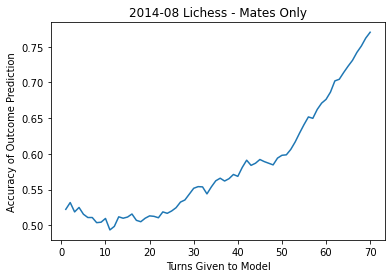
\includegraphics[scale=0.5]{0to70mates.png}
\caption{As total turns given to a model increases, so does the accuracy of a predictive model. This is as predicted, since given more of a game, one should be able to determine who would win with greater and greater accuracy.}
\end{figure}

As one can see, given more moves out of a total game, our model is able to more accurately predict the outcome of each game. Crucially, our model is relatively better than randomly guessing the outcome of the game, and can become more and more accurate given more data about the game. We predict that, given more game data (in particular, game data where only relatively good players are the opponents), we can create a model that is accurate at predicting the outcome of a chess game given a set of moves by each player.

We also predict that the accuracy of the algorithm would be improved greatly by training exclusively on the set of games played by top lever players. This might be because games played by inexperienced players tend to involve more mistakes, and thus vary wildly in who is leading the game. It is estimated that without such mistakes, the outcome of each game of professional chess is more closely tied to its beginning and so the model can anticipate less turbulence.

\section{Conclusion}
The classification of ongoing chess games is a common task for chess engines and analysers alike. While most engines and analysers look forward by predicting the best move for each player, our model simply looks at each move that the players have made so far in each game. Since engines and analysers look forward, instead of simply just looking at the turns already played, our model has the ability to quickly determine possible outcomes in times unmatched by traditional chess engines. In the future, projects like this can be used to more accurately predict the outcome of ongoing chess games, and used in complement with engines and analysers, can help people and computers become better chess players.

\section{Code Available}
The code for this project is available on GitHub at https://github.com/mryork/chesspredictor.

\section{Resources}
1. https://chessentials.com/history-of-chess-computer-engines/ \\
2. https://stockfishchess.org/ \\
3. https://database.lichess.org/ \\
4. https://dl.acm.org/doi/10.5555/1624312.1624417 \\
5. https://collaborate.princeton.edu/en/publications/explaining-adaboost

\end{document}
